\Tsec{Билет №4.1}

\begin{leftrules}
Переход от волнового уравнения к уравнениям для медленных амплитуд; разделение уравнений для волн. Решение уравнений генерации второй оптической гармоники в случае точного синхронизма. 
\\ \phantom{42} \hfill \textit{лекция 2, слайды 13-23.} 
\end{leftrules}



\setcounter{section}{4}

\begin{to_def}
    \textit{Бездифракционное приближение} -- приближение, в котором принебрегается поперечным направлению распространения расплыванием светового пучка, что влечет обнуление вторых производных по двум координатам, нормальным к координате распространения в лапласиане волнового уравнения\footnote{
        Обусловленно мили/сантиметровочными длинами рабочих нелинейных сред, а на таких длинах дифракционные эффекты мизерны
    } .
\end{to_def}

\begin{to_def}
    \textit{Медленная амплитуда} -- случай, когда волна представима произведением множителей, один из которых отвечает за быстро осциллирующую фазу, а второй за медленно изменяющуюся амплитуду.
\end{to_def}

Запищем волновое уравнение
\begin{equation*}
    \left(\cancel{\partial_x^2} + \cancel{\partial_y^2} + \partial_z^2\right) \vc{E} - \frac{1}{c^2} \partial_t^2 \vc{E} = \frac{4 \pi}{c^2} \partial_t^2 \vc{P}.
\end{equation*}
Подставляя $\vc{E}[t, z] = \vc{A}[t, z] e^{- i \omega t + i k z}$ и $\vc{P} = \sub{\vc{P}}{лин} + \sub{\vc{P}}{кв}$, находим\footnote{
    см. лекция 2, 14 слайд
} 
\textit{уравнение для медленных амплитуд}:
\begin{equation*}
    2ik \bigg( \partial_z \vc{A} + \frac{1}{v_{\text{gr}}} \partial_t \vc{A} \bigg) e^{-i\omega t + ikz} = \frac{4\pi}{c^{2}} \partial_t^2 \sub{\vc{P}}{кв}.
\end{equation*}


Использование бездифракционного приближения для медленных амплитуд позволяется убрать в волновом уравнении вторые производных по двум координатам, а оставшиеся вторых производные по координате распространения и времени свести к первым, что переводит волновое уравнение в уравнение для медленных амплитуд.



\textit{Разделение уравнений для волн:} удобно в уравнении для медленных амплитуд представить поле в видел суммы полей двух гармоник:
\begin{equation*}
    A = \frac{1}{2} (A_{\omega}e^{-i\omega t +i k_{\omega}x} + A^*_{\omega}e^{2i\omega t -i k_{\omega}x}) + \\ \frac{1}{2} (A_{2\omega}e^{-i\omega t +i k_{2\omega}x} + A^*_{2\omega}e^{2i\omega t -i k_{2\omega}x}),
\end{equation*}
после чего разделить уравнение на 2 для каждой из гармоник\footnote{
    Можно в виду тонкости спектров гармоник, которые друг друга не перекрывают, если импульсы достаточно не коротки (нано-/пикосекндные лазеры)) (слагаемые с групповой скоростью можно тоже аккуратно вычеркнуть, так как для, например, наносекундныъ лазеров их расстройка $<<$ длительности импульсов
}. В некотором приближении находим, что
\begin{equation*}
    \partial_z A \gg \frac{1}{\sub{v}{gr}} \partial_t A,
    \hspace{0.5cm} \Rightarrow \hspace{0.5cm}
\left\{\begin{aligned}
        \partial_z A_{\omega}&=\frac{2\pi i \omega}{cn_{\omega}} \chi_{2} A_{2\omega}A^*_{\omega} e^{i \Delta k z} \\
    \partial_z A_{2\omega} &=\frac{2\pi i \omega}{cn_{2\omega}} \chi_{2} A_{\omega}^{2} e^{- i \Delta k z} 
    \end{aligned}\right.
\end{equation*}



\textit{При точном синхронизме} ($\Delta k = 0$) решение уравнения для медленных амплитуд: 
\begin{equation*}
G=\frac{2\pi \omega}{cn}\chi_{2}, \hspace{5 mm} 
    \left\{\begin{aligned}
        A_{2\omega}(z) &=iA_{\omega}[0] \th\big(G A_{\omega}[0]\,  z\big) \\
        A_{\omega}(z) &=\frac{A_\omega[0]}{\ch(G A_{\omega}[0]\, z)},
    \end{aligned}\right.
\end{equation*}
таким образом на некотором расстоянии полностью переходим к $A_{2 \omega}$.
\begin{figure}[h]
    \centering
    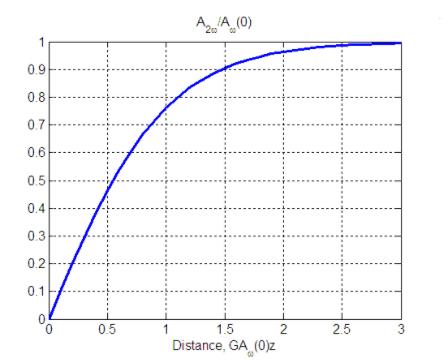
\includegraphics[width=0.3\textwidth]{figures/4_1.png}
    \caption{Генерация второй гармоники при точном синхронизме}
    %\label{fig:}
\end{figure}
